
\begin{center}\texttt{4 - Risk Mgmt}\end{center}
\hrulefill \\

\noindent We are transitioning from ``this will happen'' to ``this will \textit{probably} happen''. Risk concerns future happenings.

\noindent You should identify the risk upfront through cause-effect relations (testing takes longer (effect) because of inexperienced testing team (cause)), then you should take action to handle the possible risks, and then you should document the risk in the plan. 

\noindent Risks can involve different areas: project related (e.g. seniors turnover, change in requirements), product related (e.g. specifications are delayed or used tools are not as well-performing as thought), business risks (e.g. competitors release a product before we do).

\noindent In risk identification, you want to produce a document of many possible risks related to your prj; through risk analysis, you prioritize some risks (can't deal with all!), then you'll do planning on the reduced list (either you reduce the probability of the risk or the impact of it, so either the cause or the effect); then, you do risk monitoring while the project unfolds. The process of risk management is iterative, risks change in priority and relevance through the life cycle of the prj!

\noindent The main identification techniques is simply checklists (others' experiences) and brainstorming (your experience).

\begin{figure} [H]
    \centering
    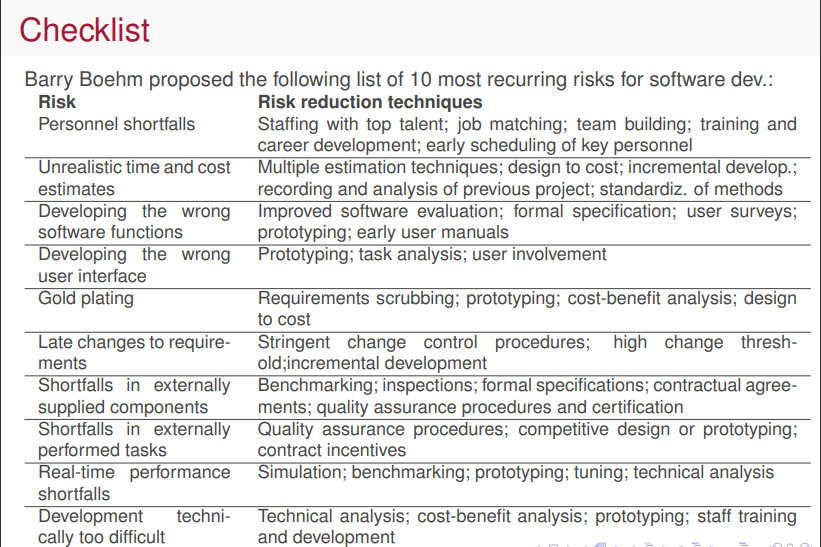
\includegraphics[width=0.75\linewidth]{Figures//04/checklist.png}
    \caption{Checklist of the 10 most frequent risks up to some years ago.}
\end{figure}

\begin{figure} [H]
    \centering
    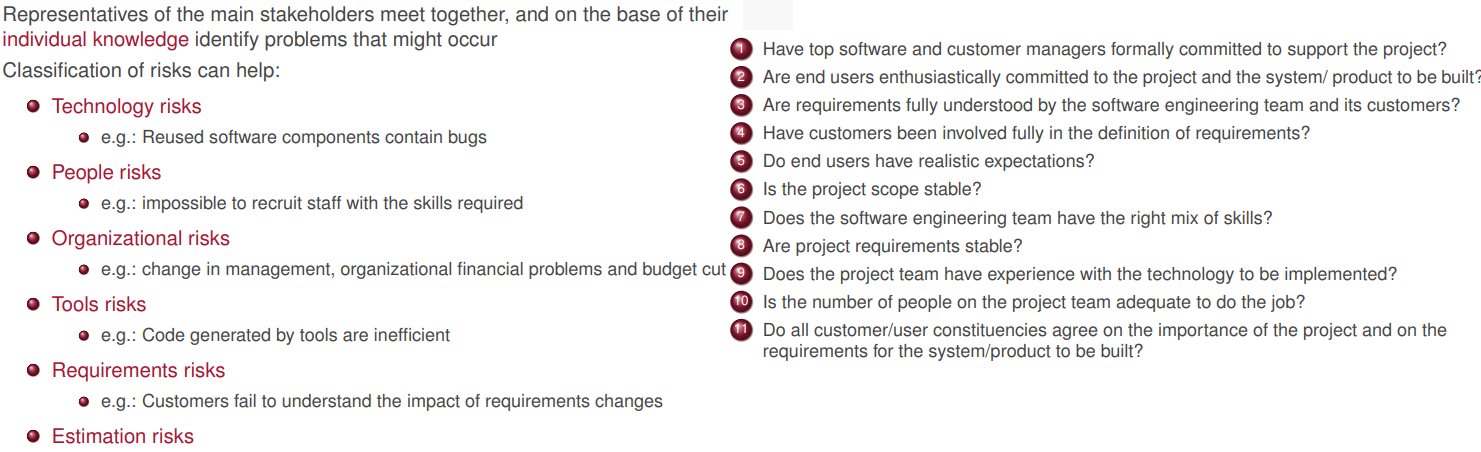
\includegraphics[width=1\linewidth]{Figures//04/bs1.png}
    \caption{On Brainstorming.}
\end{figure}

\noindent Risk analysis: you want to rank the top risks by some factors, such as probability of occurrence and impact of occurrence: Risk Exposure $=$ potential damage $\times$ prob of occurrence. You rank those and pick the higher ranking one.

\noindent Or you go for a more approximative approach, which is the $4 \times 4$:

\noindent Build a $4 \times 4$ matrix in which columns represent Probability of risk happening: Low ($<10\%$), Moderate ($10\%\div29\%$), Significant ($30\%\div50\%$), High ($>50\%$); rows are impact of the risk if it manifests: Insignificant ($<10\%$ on budget), Tolerable ($10\%\div19\%$ on budget), Serious ($20\%\div29\%$ on budget), Catastrophic ($>30\%$ on budget). Select a number between 2 and 8 and mark the cells according to this number, all the risks that are above said threshold.

\begin{figure} [H]
    \centering
    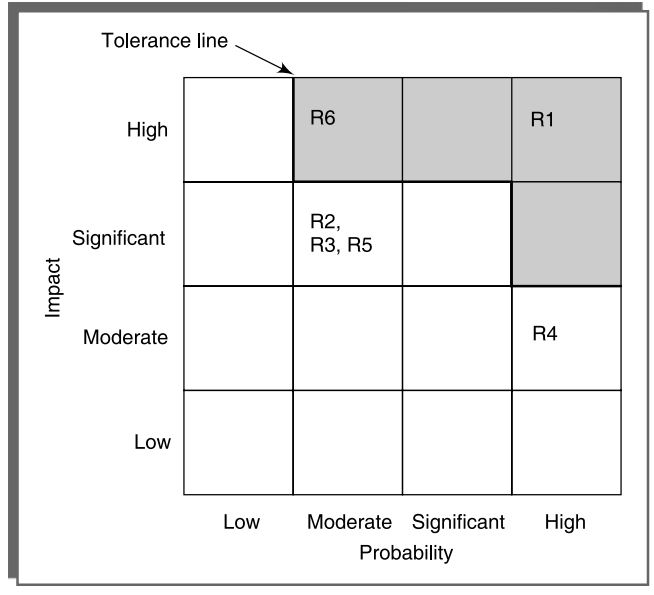
\includegraphics[width=0.5\linewidth]{Figures//04/4x4.png}
    \caption{A Probability Impact Matrix.}
\end{figure}
\newpage

\noindent When faced with risk, you could deal with it:
\begin{itemize}
    \item acknowledge: ehh it's there *shrug*;
    \item avoidance: review the action so that the risk can no longer occur (IDE is buggy? change IDE);
    \item transfer: perhaps outsource the risky task to another agent, so that the risk becomes their responsibility;
    \item risk reduction and mitigation techniques.
\end{itemize}

\noindent Reduction and mitigation:
\begin{itemize}
    \item Reduction: act on reducing the probability of happening. You want to look at Risk Reduction Leverage: \[RRL = \dfrac{RE_{before}-RE_{after}}{CostOfReduction}\]
    if this ratio is greater than 1, it means that it's better to apply the reduction than to run the risk, so we reduce it, else we don't. Think of the salary improvement over a year example;
    \item Mitigation: act on reducing the impact of the risk happening. Staff can get sick? Make sure to have overlapping of work among people, so that everyone can potentially cover for the sick! 
\end{itemize}

\noindent Contingency Plan: the ``Plan B'' for high-relevance risks, the detailed plan on what to do in case the risk occurs.

\noindent Monitoring: (at runtime) look out for any misalignment with the plan and try to understand

\noindent \underline{PERT}: Program Evaluation and Review Technique, define the schedule of activities taking into account uncertainties in the duration of it - a reasonable delay, the probable realistic duration if likely trouble occurs.

\noindent In PERT, you will have a three-point assessment: most likely time est. (m), optimistic time (a), pessimistic time (b). The expected duration is a weighted average that goes:
\[t_e = \dfrac{a+4m+b}{6}\]

\noindent implying that the best case is as likely as the worst: neither of them is that likely, far less likely than the likely one, lmao duh. Standard deviation goes:

\[\sigma = \dfrac{b-a}{6}\]

\noindent PERT analysis: on an activity-on-arrow graph, we report the expected duration on each node, but also the accumulated uncertainty. The more you proceed through the graph, the more you will accumulate uncertainty. What's the accumulated uncertainty of a whole path?

\noindent People tend to work on deadlines, i.e. Parkinson's law, for very natural reasons, and from what I gathered the PERT analysis per se does not take into account this phenomenon, but such a shortcoming seems to be mitigated by the application of the Critical Chain approach - we'll see, I guess.

\noindent For each activity, we're going to have three estimated times: $m$, $a$, $b$.

\begin{figure} [H]
    \centering
    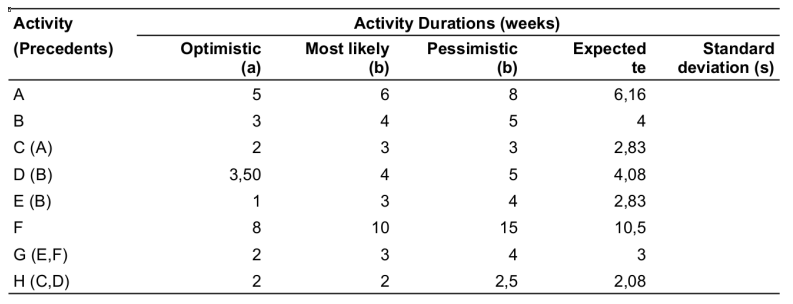
\includegraphics[width=0.75\linewidth]{Figures//04/pert00.png}
    \label{fig:pert_table}
\end{figure}

\noindent Some prob theory: Random variable is a value from a pool with a certain probability of being extracted, if this P is uniform then every value from the set of possible values has the same probability of happening (e.g.: roll the dice). From a distribution you can derive the expectation, which is the arithmetic mean of the possible values a random variable can take, weighted by the probability of those outcomes. In the case of symmetric distribution (e.g.: Gaussian bell), the expectation is the exact ``middle'' value. The deviation $\sigma$ is basically how much a value deviates from the expectation, it gives you how far the values are actually distributed from the expectation point.

\noindent We will consider $t_e$ as our expectation and $\sigma$ as the uncertainty coefficient, basically, how uncertain is this estimation.

\noindent We don't want to make precise computations because our initial data itself is approximated anyway, an estimation itself.

\noindent Table \ref{fig:pert_table} contains the initial information for all our activities. Now we want to derive numbers for paths of activities!


\noindent How to minimize the number of nodes: reflect on the dependencies, those are the ones that cause the most clutter. You could redirect the nodes that end before the longest one to the longest lasting one, then from this node you go forward. If no node needs such information about which node ended, you can redirect it to the next useful node. But you gotta be careful not to introduce the wrong dependencies as you do so! Reason on dependencies.

